\documentclass[12pt]{article}
\usepackage{amsmath}
\usepackage{emptypage}
\usepackage{blindtext}
\usepackage{titlesec}
\usepackage{float}
\usepackage[hidelinks]{hyperref}
\usepackage{graphicx}
\usepackage[italian]{babel}
\graphicspath{ {./images/} }
\author{}
\title{
    \huge 
        \textbf{Università degli Studi di Modena e Reggio Emilia}
    \large
        \par Dipartimento di Scienze Fisiche, Informatiche e Matematiche
        \par Corso di laurea in Informatica
    \vfil
        \huge \par \textbf{Engim report service}
    \vfil
    \normalsize
    \begin{tabular}{lp{0.4\textwidth}l}
      Relatore: & & Candidato: \\
      Prof. Claudia Canali & &  Dumitru Frunza \\
      \end{tabular}
}
\date{Anno academico 2021/2022}
\linespread{1.5}



\begin{document}
\maketitle
\thispagestyle{empty}
\newpage 
\thispagestyle{empty}
\
\newpage
\pagenumbering{roman}
\addtocounter{page}{0}
\listoffigures
\newpage
\phantomsection
\tableofcontents
\addcontentsline{tesi}{Infrastruttura}{Infrastruttura}
\newpage
\pagenumbering{arabic}
\addtocounter{page}{0}


\phantomsection
\section*{Introduzione}
\addcontentsline{toc}{section}{Introduzione}
Un software gestionale è un sistema creato per aiutare un'azienda a organizzare 
e gestire il lavoro.
Engim offre la possibilità di monitorare le mansioni di un lavoratore e garantire 
la sua sicurezza tramite ServizioGPS e TwiceTouch, i due prodotti di punta dell'azienda. 
In particolare, servizioGPS salva il percorso di una macchina lavoratrice e 
permette di calcolare il contributo dovuto. Ogni via attraversata viene salvata, 
ogni 5 secondi viene salvata una coordinata GPS.
\\ Nell'affrontare una grande quantità di dati, diventa importante
 disporre di un metodo affidabile e intuitivo per l'archiviazione degli stessi.
Un modo comune per salvare informazioni è tramite un file XLSX o PDF.
I file PDF sono semplici da usare, interpretare e sono estremamente diffusi 
rendendoli perfetti per un cliente senza capacità tecniche. 
Un servizio simile può essere parte integrale del software in quanto effettivamente 
è un estensione di esso.
Questo è vero fin tanto che richiede minime risorse e tempo di calcolo.
\\ Cosa succede quando un servizio secondario, importante per i clienti ma non 
abbastanza da giustificare un grosso impegno da parte del server, pesa gravemente 
sul software? 
È il problema che sta affrontando Engim; il servizio di conversione di dati 
in PDf richiede troppe risorse per periodi prolungati rendendo difficile la user 
esperienze ma soprattutto sovraccaricando il server.
Intuitivamente si potrebbe migliorare la situazione attuale, andando a riscrivere 
il codice incriminato.
Una soluzione che però risolve solo il problema in termini di tempo e non di 
risorse, resta comunque un processo potenzialmente gravoso sulla macchina. 
Un altro possibile approccio sarebbe quello di delegare il calcolo.
\\ È possibile effettivamente astrarre il processo di conversione, portarlo su 
un servizio di terze parti migliorando performance e risparmiando risorse.

\thispagestyle{empty}
\newpage 
\thispagestyle{empty}
\
\newpage

\section{Engim Srl}
\subsection{L'azienda}
Engim è una società che si occupa di creare soluzioni tecnologiche in ambito 
ICT, telecomunicazioni, sistemi di gestione e mobilità. Da oltre 10 anni operano 
nel mercato della tracciabilità di flotte e attività e della 
sicurezza dei lavoratori in solitario.
\\ ServizioGPS è il noleggio di tracker GPS per veicoli lavoratori. 
Una prevalente parte dei clienti sono comuni che, tramite i prodotti Engim, 
tracciano il percorso delle macchine spazzaneve e spargisale.
I tracker possono essere prodotti fisici oppure un app per smartphone. A loro 
volta i prodotti fisici si dividono in fissi e mobili. Il servizio include
anche un gestionale per poter visualizzare, modificare o archiviare i propri dati.

\begin{figure}[H]
\includegraphics[scale = 2]{dispositivi.jpg}
\centering
\caption{Servizi disponibili}
\end{figure}
Come è possibile osservare dalla figura, noleggiando uno qualsiasi dei dispositivi 
servizioGPS è possibile avere un resoconto dettagliato del percorso effettuato 
dai lavoratori anche in tempo reale. 
Inoltre garantisce della sicurezza extra monitorando lo stile di guida e 
possibili furti o incidenti. 

Twicetouch è noleggio di dispositivi di sicurezza individuale.
Il prodotto tutela i lavoratori in solitario mandando una segnalazione in caso di
emergenza. Esistono due tipi di rilevazione: 
\begin{itemize}
  \item caduta: l'accelerometro del dispositivo rileva un urto pericoloso
  \item assenza di movimento: il lavoratore non si è mosso per un lasso prolungato di tempo, 
  quindi si presume che possa essere incosciente
\end{itemize}
Similmente a servizioGPS è possibile noleggiare un dispositivo fisico (badge) oppure
l'app per android. In entrambi i casi è possibile impostare i numeri in caso di 
emergenza, che riceveranno una chiamata e un messaggio SMS.

\subsection{Infrastruttura}
Le tecnologie usate per servizioGPS sono le seguenti:
\begin{itemize}
  \item Ruby on rails full stack
  \item MariaDB, Redis  e DynamoDB come database
  \item Python come backend di supporto
  \item Java per il prodotti app 
\end{itemize}
\begin{figure}[H]
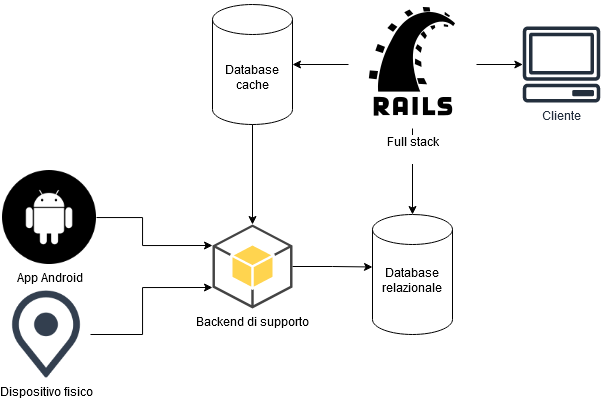
\includegraphics[scale = 0.6]{infrastructure.png}
\caption{Architettura}
\end{figure}
Ruby on Rails è usato per front-end e gran parte del backend di servizioGPS. 
Qualsiasi necessità front end side è responsabilità di Rails, questo è dove 
viene svolto la maggior parte della manutenzione siccome ha molte servizi diversi 
ed è a stretto contatto con il cliente.
\\ Il "Fetcher" (backend di supporto) invece si dedica esclusivamente alla elaborazione
di coordinate GPS. 
Questo non si trova sullo stesso server di Rails, bensi sul suo privato, molto 
più potente siccome svolge una funzione vitale per il gestionale.
Avendo poche funzionalità tende ad avere bisogno di una minore 
manutenzione.
Inoltre il servizio si appoggia su molteplici server. 
Non è importante quanto potente possa essere la macchina, con decine o addirittura 
centinaia di migliaia di punti, si corre un grosso rischio tenendo un singolo 
calcolare.
\\ I dati vengono salvati in un database relazionare MariaDB e utilizza come 
servizi di cache Redis e DynamoDB. 
\\ Ogni app è sviluppato in android nativo e lavora tramite chiamate API 
con il suo server designato. 

\subsection{Sistema automatico di generazione di report}
Engim esegue una manutenzione annuale di database, che consiste nell'archiviazione
dei dati del periodo specifico.
Questi possono essere salvati dal cliente, nel caso fosse interessato 
o necessitato, sotto forma di PDF oppure XLSX.
\\ 
Le informazioni più importanti sono l'elenco e le specifiche di tutte le "attività". 
Un'attività contiene una serie di dati, tra cui: coordinate
GPS, costi di lavoro, tempo di lavoro e altro.  
Al momento il servizio è implementato da Rails tramite una libreria di ruby. 
Il sistema attuale crea un istanza di chrome, l'istanza contiene un HTML
che si desidera convertire in PDF e infine avviene il parsing del documento.
\\ Questo ha una serie di gravi problemi:
\begin{itemize}
  \item La necessità di avviare un istanza di chrome e il parsing di un HTML è
  estremamente costoso dal punto di vista delle risorse
  \item Il parsing di un HTML è anche estremamente costoso in termini di tempo,
  aggravato dalle lunghe query dovute alla grande mole di dati 
  \item Il  parsing tende a essere poco affidabile
  \item È necessario avere delle pagine HTML nel codice che effettivamente 
  non vengono usate ma servono solo alla stampa 
  \item L'operazione causa relativamente spesso crash, perché il server 
  per il frontend non è adatto a operazioni impegnative
\end{itemize}
Il problema sicuramente si potrebbe attenuare direttamente nel frontend. 
Ad esempio facendo una misurazione di performance per vedere quali 
miglioramenti è possibile fare, ma questo non risolverebbe la richiesta di risorse. 
C'è un alternativa molto più valida.
\\ La natura del nostro problema sembra perfetta per il cloud computing.
L'operazione è ripetitiva, ben definita e usata per brevi periodi. Altri vantaggi 
importanti sono il risparmio di risorse del server, che evita di gravare sulle 
operazioni più critiche, e la possibilità di usare il progetto per qualsiasi 
altro prodotto Engim.

\section{Cloud computing}
\subsection{Introduzione}
Il cloud computing è una serie di servizi on-demand, generalmente di archiviazione 
e potenza di calcola. 
L'utente cede, in parte o totalmente, il controllo sul sistema a sua disposizione, 
evitando la manutenzione necessaria per le macchine fisiche.
Il servizio viene erogato con un modello pay-as-you-go, ovvero si paga l'effettivo 
utilizzo invece che una quota fissa per un determinato periodo. 
Questo approccio potrebbe aiutare a risparmiare soldi, soprattutto durante 
la fase iniziale di investimento, siccome non richiede pagamenti di attivazione.
Allo stesso tempo si è in balìa del provider, se le richieste dovessero 
aumentare notevolmente ci si potrebbe ritrovare con una spesa enorme.
È un rischio che le grandi aziende sono felici di correre, infatti nel 2023 il 
mercato del cloud computing ha un valore di 706 miliardi. Si stima che entro il 
2025 il numero crescerà fino a 1.8 bilioni. 
\\ L'idea di condividere risorse non è nuova, infatti nasce nel 1960. Al tempo 
un ufficio aveva un mainframe con varie postazioni. Ogni macchina poteva fare 
una richiesta tramite un job e doveva aspettare l'esecuzione del computer 
centrale: \textbf{remote job entry}.
\\ Nel 1990 le aziende di telecomunicazioni sono passate da connessioni 
point-to-point a virtual private network.
La performance non ha subito alcun miglioramento ma adesso era possibile 
decidere come impiegare le risorse. I clienti ricevevano banda in base 
alla loro richiesta, questo risultava in un grosso risparmio per l'azienda.
\\ Il pioniere del cloud computing come lo conosciamo oggi è stato Amazon che 
nel 2002 ha lanciato Amazon Web Services.

\subsection{AWS}
Amazon Web Services è una sussidiaria di Amazon che offre servizi di cloud 
computing e APIs per individui, aziende e governi.
Il più popolare è Amazon Elastic Compute Cloud (EC2), 
un cluster di computer usabili tramite REST API, CLI o AWS console.
È il corrispettivo di un server tradizionale nel contesto del cloud computing. 
EC2 supporta una vasta gamma di processori, dai più tipici come Intel e AMD, 
fino ad Arm per l'architettura macOS.
Ogni componente simula il comportamento della sua controparte fisica, permettendo 
l'aggiunta e la rimozione di tale unità. 
L'utente può quindi personalizzare la macchina a suo piacimento. 
\\ Di frequente questo servizio viene usato in coppia con Amazon CloudWatch,
il quale ha lo scopo di monitorare CPU, archiviazione e rete, e quando fosse 
necessario aumentare le risorse.
Il sistema ogni minuto, oppure secondo, può scegliere se allocare più 
potenza.
Il cliente può quindi abbandonare l'allocazione manuale di risorse, il server 
pensa a tutto e addebita in base ai componenti usati in ogni determinato momento. 
Non è più necessario avere qualcuno che manualmente, nel momento del bisogno, 
cambi le caratteristiche della macchina.
\\ Il server può essere di natura tradizionale o "istance-store". 
Un istanza viene creata ogni volta che avviene un deploy, questa istanza è 
unica e non è fissa.
Nel secondo caso non appena l'istanza si ferma, sia per un malfunzionamento 
ma anche per un banale riavvio, ogni dato salvato in locale verrà perso. 
Ovviamente si hanno a disposizione una serie alternativa di unità di archiviazione.

\subsection{Archiviazione}
Amazon Elastic Block Store (EBS) simula l'aggiunta di un unità di memoria di 
massa fino a 16 TiB per ogni volume. 
È possibile utilizzarne molteplici, proprio come in un computer fisico, ma con 
un vantaggio importante: ogni volume ha almeno un backup. 
Il fallimento di un singolo componente non compromette il sistema.
\\ Non sempre è necessario gestire una memoria così complessa, ma è sufficiente 
avere uno spazio, simile a google drive, dove salvare alcuni file multimediali.
Amazon S3 è un servizio di archiviazione di oggetti veloce e scalabile. 
Tale locazione è accessibile da qualsiasi piattaforma e si paga in base allo 
spazio utilizzato.
\begin{figure}[H]
\includegraphics[width = \textwidth]{bucket.png}
\centering
\caption{Schema di un bucket}
\end{figure}
Come si evince dall'immagine S3 permette a qualsiasi genere di applicazione 
l'accesso alla memoria. 
Una volta salvato il file è possibile scaricalo tramite lo stesso servizio 
oppure un altro e persino analizzarlo.
\\ Rispetto a EC2, S3 non richiede la conoscenza o gestione della tecnologia 
sottostante, è tutto in mano al provider.
Tecnologia che si sposa molto bene con i microservizi

\subsection{Microservizi}
Un passaggio ulteriore verso il cloud computing è quello di non avere nemmeno 
un sistema operativo o un ambiente di sviluppo.
Le lamda sono funzioni salvate su piccole unità di memoria dormiente. 
Quando viene ricevuta una richiesta HTTPS, l'ambiente verrà creato e la 
funzione eseguirà. 
\\ Il costo dipende dal tempo di esecuzione unito alla potenza della macchina 
da virtualizzare. 
Non si ha alcun controllo sul sistema operativo, ne alcun altro aspetto 
dell'ambiente.
È possibile sviluppare un blocco logico e portarlo in produzione in maniera 
estremamente facile, ma avendo il limite delle tecnologie compatibili.
\\ Il vantaggio di tale operazione è quello di prendersi carico del calcolo 
necessario, liberato risorse preziose dal proprio server. 
Lo spazio di archiviazione disponibile è il minimo necessario per salvare il 
codice, qualsiasi altro file va salvato su un altro servizio.
\begin{figure}[H]
\includegraphics[width = \textwidth]{lambda.png}
\centering
\caption{Esempio di lambda unito a s3}
\end{figure}
Un semplice esempio di lambda che utilizza S3 come spazio di archiviazione. 
In questo caso l'utente richiede un informazione particolare e la lamda 
va a trovare tale informazione da DynamoDB. 
\\ Nel caso in cui sia necessario compiere un operazione raramente o in maniera 
discontinua, lambda sembra essere un eccellente opzione. 
Il sistema ha un tempo di ritorno maggiore alla prima chiama (cold start)
che per un tempo limitato viene evitato, dopo il primo avvio.
Naturalmente non è una tecnologia adatto a ogni caso d'uso. 
Un servizio è la scelta corretta 
quando serve una risposta immediata o sia necessario un esecuzione continua.

\section{Requisiti del progetto}
\subsection{Descrizione}
Il progetto è una funzione lambda su AWS, ovvero un microservizio.
Il modo più semplice per eseguire tale codice è attraverso una chiamata 
HTTPS, nel caso di questo progetto è una POST, siccome prevede l'invio di dati.
La funzione viene chiamata in maniera diretta tramite una libreria di ruby.
Questa richiede le credenziali IAM per effettuare l'accesso alla lambda e prende 
in input un JSON. Al suo interno abbiamo un token di autenticazione e il dominio 
di provenienza che vengono controllati dalla lambda. 
\\ I contenuti invece sono divisi in sezioni per permettere dinamicità di stampa, 
qualora uno dei blocchi fosse assente, semplicemente non verrà stampato. 
\\ Nel caso in cui la stampa sia avvenuta correttamente la funzione ritorna 
"200 OK"
e il nome del file su S3. Se l'input della chiamata risulta errato, la funzione ritorna 
"400 BAD REQUEST"
e un messaggio che descrive l'errore. Infine se avviene un errore di connessione 
al bucket S3, la funzione ritornerà un errore "500 INTERNAL ERROR".    
\\ Il progetto deve permettere l'implementazione di stampe diverse da quelle di servizioGPS
e di altri file di output come KML e XLSX. 

\begin{figure}[H]
\includegraphics[width =\textwidth]{realUseCases.png}
\caption{Casi d'uso}
\end{figure}
I casi d'uso sono molto semplici, siccome una lambda è pensata per essere 
un singolo blocco logico, deve effettuare una singola funzione.
L'utente può richiedere la visualizzazione di una stampa oppure il diretto 
download. La funzione esegue il parsing dei dati.


\subsection{Sicurezza}
L'autenticazione avviene a livello di codice, sia sul server che sul microservizio.
\\ La libreria \textit{aws-sdk-lambda} permette di stabilire una connessione diretta con la 
lambda.
È sufficiente fornire: nome della funzione, regione, credenziali e payload. 
Le credenziali sono una coppia di token sicuri e 
sono salvati dentro un file crittografato yaml. 
Al momento del bisogno il framework può decodificare tale file e 
leggere le informazioni. 
La chiave per decrittare il file è caricata manualmente sul server destinatario.
\\ Un ulteriore livello di sicurezza è integrato nella funzione sotto forma 
di token e whitelist. 
Questi valori sono salvati nel ambiente di AWS, in maniera simile al file 
crittografato in precedenza. 
L'ambiente viene creato con queste variabili salvate, e nel momento del 
bisogno possono essere lette, evitando di doverle scrivere a mano nel codice.
Il token è un lungo carattere alfanumerico.
La whitelist contiene tutti i domini di Engim, questi vengono caricati in 
una lista e confrontati con il mittente. 
Non vengono accettate richieste senza specificare il server di invio.
Nel caso in cui l'operazione sia andato a buon fine, ritornerà un JSON in risposta.
\\ Qualsiasi chiamata da dominio esterni oppure senza token verrà tratta come 
"400 BAD REQUEST". 

\subsection{Correttezza dei dati}
Esistono 3 blocchi principali: "header", "body", "table".
Fin tanto che almeno uno dei 3 è presente, la stampa risulta valida.
Facoltativamente è possibile includere il blocco "media", che contiene 
eventuali immagini in "base64". 
\\ Il header può contenere fino a 2 loghi, però deve necessariamente avere 
un titolo e una intestazione. 
Uno dei due loghi è sempre quello aziendale, mentre l'altro può essere una copia 
del precedente oppure appartenere al cliente.
L'intestazione racchiude: dominio di provenienza, nome utente e data di oggi.
\\ Il body può avere un numero arbitrario di blocchi. Ogni blocco è racchiuso 
in un rettangolo e anche esso ha una serie di titoli con i loro dati. 
È valida l'assenza di un dato, ma invalida l'assenza di un titolo. 
\\ Il table è composto da una serie di titoli e una serie di righe. Non c'è limite 
al numero di righe che può contenere.
Anche in questo caso non può mancare un titolo ma un dato può essere vuoto. 
\\ Tra i tipo di dato, di una tabella, 
è possibile avere un immagine che viene spedita in 
base64, se è assente non verrà scritto nulla. Onde evitare la duplicazione 
eccessiva di immagini, siccome una tabella potenzialmente contiene un numero 
elevato di dati, le immagini sono salvate nel blocco media in singola coppia. 
\\ Il programma presume che i dati siano corretti, controlla solo la loro presenza.
La funzione anche presume che ogni dato sia una stringa, questo evita conversioni 
e permette di stampare qualsiasi dato a prescindere dalla provenienza.

\subsection{Problemi interni del server}
Durante l'esecuzione vengono effettuate delle connessioni dirette tra i servizi. 
In un primo momento Rails si collega con la lambda, questa connessione potrebbe 
essere soggetta a timeout. 
C'è un limite di tempo di calcolo in modo da evitare loop infiniti.
\\ Lambda a sua volta crea un canale con il bucket, per poter 
effettuare il caricamento del file, qualsiasi tipo di errore viene catturato da javascript.
Nel caso in cui il file venga salvato correttamente,
la lambda restituisce la chiave del file, ovvero il suo nome. 
\\ Infine Rails si collega al bucket e cerca il link per aprire o scaricare il file 
direttamente dal bucket.
Questa connessione può sembrare superflua, ma aggiunge 
un livello di sicurezza ulteriore senza aumenti degni di nota sul costo temporale. 


\subsection{Presupposti e dipendenze}
Siccome AWS mette a disposizione l'infrastruttura c'è una scelta limitata dei 
linguaggi di programmazione.
Nella lista sono presenti i più popolari al momento,
in particolare sono stati presi sotto esame python, ruby e javascript.
\\ Ruby ha numerose librerie che permettono la scrittura dei PDF che purtroppo
prevedono il parsing di un HTML.
Questa operazione è molto vantaggiosa per lo sviluppo ma non particolarmente 
per l'efficienza.
Ogni conversione richiede un istanza di chrome da cui convertire il file,
creando una serie di processi non necessari.  
\\ Python offre molteplici librerie, ognuna con diverse funzionalità. Non è 
sufficiente usarne sol una per le operazione desiderate e inoltre 
molte di queste librerie non sono mantenute in maniera costante
\\ Javascript invece ha "pdfkit", una libreria che permette la creazione e manipolazione 
di un PDF senza intermezzi. È molto popolare, open source con una comunità 
attiva, oltre ad avere una documentazione breve e chiara.
\\ La stampa ha una forma regolare, divisa per righe e colonne. Se i dati sono 
disposti in maniera più arbitraria è necessaria un implementazione diversa. 
Non è richiesto la stampa in altri formati di file, ma è necessario lasciare 
la libertà di aggiungere diversi formati in futuro.

\subsection{Features}
La lambda ha un unica funzionalità, stampa e salvataggio della stampa.
\begin{figure}[H]
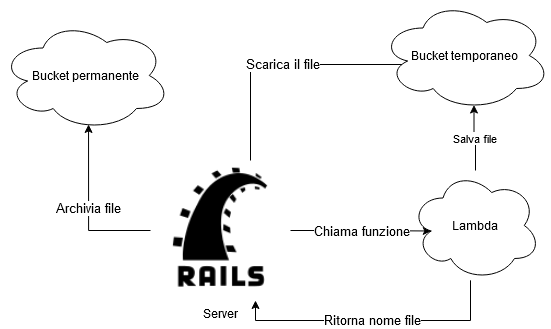
\includegraphics[scale = 0.6]{useCases.png}
\caption{Schema logico}
\end{figure}
Ogni stampa deve seguire seguire lo schema a blocchi definito, non è possibile 
ad esempio affiancare un immagine in una tabella. 
Qualsiasi implementazione che non segua lo standard va aggiunta alla funzione.
\\ È possibile stampare immagini che devono essere prese in input siccome non 
esiste una memoria permanente per la funzione.
\\ Ogni file viene salvato su lambda, il nome univoco di ogni file è 
data e ora di quel esatto istante. 
S3 crea automaticamente cartelle divise per mese e per giorni. 
Una volta che il file è stato salvato, Rails può trovare il file e mostrarlo 
oppure scaricarlo per l'utente.
\\ Il bucket temporaneo viene svuotato periodicamente, se un dato serve per il 
cliente verrà salvato sul bucket permanente, 
altrimenti nel tempo verrà cancellato.
\\ Il motivo per la divisione dei bucket è per dividere la logica, 
la lambda non ha l'obiettivo di organizzare un bucket.



\section{Implementazione}
\subsection{Flusso di lavoro}
È stato deciso di lavorare con continua integrazione. 
\\ In prima battuta creare una funzione in grado di generare un PDF e salvarlo 
su S3. Testare ogni aspetto della funzione ed effettuare il deploy su AWS. 
\\ Successivamente integrare la funzionalità in rails, eliminando la vecchia 
funzione. Assicurarsi che la stampa esegue correttamente ed in tempi ragionevoli.
\\ Al termine dell'implementazione verrà effettuato un deploy su un server 
di staging. Dopo un breve periodo di test, sarà possibile portare la modifica 
su un server di produzione. L'integrazione partirà da un server per effettuare 
test aggiuntivi e infine raggiungera i restanti.
\\ Ogni deploy è effettuato attraverso Gitlab usando le pipeline. 
Definendo un file .gitlab-ci è possibile eseguire una serie di operazioni 
bash-like. 
Nel caso della lambda la pipeline compie i seguenti passaggi: 
\begin{itemize}
  \item Crea un ambiente immagine da usare come ambiente di sviluppo 
  \item Installa tutte le dipendenze specificati nel nostro pacchetto
  \item Esegue tutti i test automatizzati 
  \item Se tutto funziona correttamente esegue il deploy, altrimenti avverte 
  che la pipe ha fallito
\end{itemize}

\subsection{Creazione di un file e salvataggio su S3}
È possibile interagire con un bucket S3 tramite due modi: connessione con link 
creato da un utente autorizzato oppure connessione IAM. In questo particolare 
caso è necessario stabile una connessione diretta tramite IAM. Una volta stabilita 
è possibile accedere a una serie di metodi tra cui "upload()". Al termine del 
caricamento il bucket ritorna un dizionario con una serie di informazioni, la 
più importante è la chiave, che è il nome del file su S3. Nota importante, 
non usare "key" perché è un valore vecchio per retrocompatibilità, bensi "Key". 
Il primo valore è poco affidabile, potrebbe essere vuoto nonostante l'oggetto 
esista.

\subsection{Generazione di un PDF da un JSON}
La libreria permette scrittura sul file, disegno elementare e manipolazione di 
font, posizione e colore.
Inizialmente appariva conveniente un approccio funzionale, ma vedendo il modo 
particolare in cui viene esportato un file in "Nodejs" e la complessità sempre 
maggiore dei documenti, è stato deciso di creare una classe: PdfDocument. 
\\
Il costruttore va a definire la grandezza del documento in base al blocco più 
largo del file.
Questa definisce la larghezza del documento e l'altezza viene calcolata di
conseguenza (1.41 volte più grande, come un foglio A4).
Il formato default è A4, per evitare stampe troppo piccole.
Mantenendo queste proporzioni la visualizzazione e la stampa risultano molto 
semplici.
Una volta definito il documento la classe chiama il metodo "writeData()".
Questo controlla la presenza dei dati e richiama altri metodi di scrittura 
se necessario.
I metodi di scrittura controllano che non manchino dati vitali e se così non fosse 
scrivono sul documento. 
È possibile richiedere il documento tramite "getDocument()". 
\\ Il file è uno stream di dati e può essere spedito direttamente su S3. 

\begin{figure}[H]
\includegraphics[]{uml.png}
\centering
\caption{UML}
\end{figure}
Struttura del file-classe lambda. 
Una singola classe che crea 3 variabili a livello di costruzione da usare 
all'interno di ogni istanza del oggetto. 
La maggior parte dei metodi sono funzioni di scrittura direttamente 
nel file PDF.
Eccezione fatta per documentWidth() che calcola la larghezza del file in base 
all'input e getDoc() che ritorna il file. 

\subsection{Test automatizzati}
Si è deciso di effettuare del "unit testing" tramite la libreria mocha.
In un file separato viene generato un evento valido per la lambda.
Ogni dato dell'evento è generato in maniera casuale tramite "faker-js". 
Naturalmente questi dati hanno una serie di limitazioni per poter essere 
casuali ma al contempo validi per lo scopo. 
Sono stati quindi effettuati una serie di test di sicurezza, generando 
richieste valide e invalidi, una per ogni tipo di errore. 
È stato anche fatto una serie di test dove veniva verificato l'input. 
Partendo dal evento valido, vengono rimosse informazioni importanti e ci si 
aspetta un errore di ritorno.
Infine le connessioni con AWS sono simulate tramite "aws-sdk-dev". 

\subsection{Ruby on Rails}
Il metodo di stampa corrente ritorna una pagina HTML e richiede la stampa oppure 
scarica la conversione di quella pagina. Innanzitutto è necessario cambiare il 
ritorno da HTML a PDF e in seguito passare un valore alla chiamata per distinguere 
la visualizzazione dallo scaricamento del file. 
La prossima fase è caricare tutti i dati in un hash e trasformarlo in un JSON. 
Ogni stampa ha disposizioni simili ma una conversione dei dati diversa, è quindi 
necessario creare due distinte funzioni: una per le attività e una per la singola 
attività
\\ Una volta definito il JSON si può stabile una connessione diretta con la lambda e 
chiamare il metodo interessato.
Al termine della chiamata il metodo ritornerà il nome del file e stabiliamo un
ulteriore connessione, stavolta col bucket, per visualizzare o scaricare il file.
Il ritorno di questa richiesta è un JSON che
contiene una serie di link tra cui il url di download e il url di visualizzazione.
Il motivo per cui questo non viene ritornato direttamente dalla lambda è per avere 
un livello di sicurezza extra. 

\section{Applicazione e performance}
\subsection{Risultati}
Non è stato necessario cambiare nessuna parte dell'interfaccia grafica.
Sul nav della sinistra sono presenti una serie di funzioni di servizioGPS, 
l'unica di nostro interesse è Activities, e una serie di dati extra. 
Il primo grosso blocco è un classico blocco di ricerca che permette 
di trovare attività specifiche.
È possibile stampare una lista di attività cliccando sulla stampante oppure una 
scaricarle cliccando sul immagine alla sua destra, infine è possibile spedirle 
per mail tramite la lettera. 
Il blocco sottostante è un riassunto delle attività, è compreso nella stampa. 
Infine segue una tabella con tutti i dati importanti: id, stato, 
prima posizione, ultima posizione, tipo, dispositivo, utente, 
azienda e servizio in totale. 
\begin{figure}[H]
\includegraphics[width =\textwidth]{lista_attività.jpg}
\caption{Lista di attività}
\end{figure}
Di seguito è possibile vedere un esempio di stampa di attività. 
In alto è possibile trovare il server di provenienza, con tanto di data e 
azienda.
A destra è scritta la versione del software della lambda. 
Il header è il blocco con il titolo e il logo di servizioGPS.
Il body è il blocco che riassume il blocco visto nell'immagine precedente. 
Il table è l'elenco di tutte le attività, che è identico a quello sul server, 
esclusa l'ultima posizione.
In questo caso sono presenti 6 attività, ma possono essere fino a 20 mila. 
\begin{figure}[H]
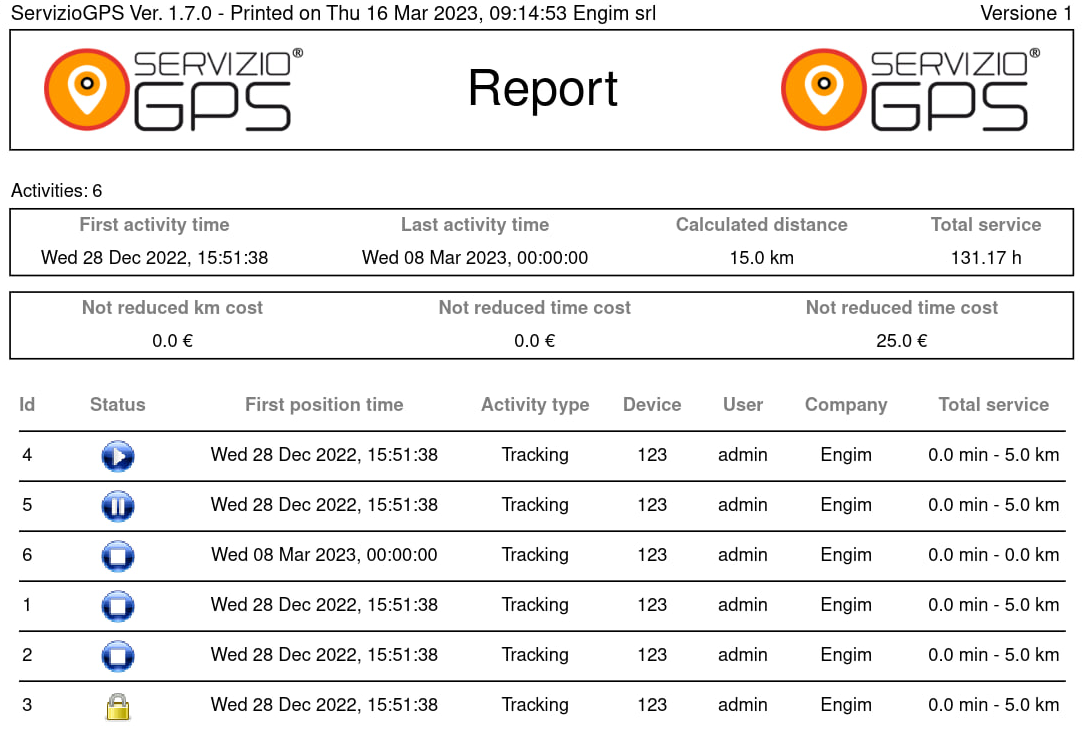
\includegraphics[width =\textwidth]{report.png}
\caption{Stampa del elenco attività}
\end{figure}

Alternativamente è possibile stampare i dettagli di un unica attività. 
In questa pagina è possibile vedere nel dettaglio il percorso fatto 
dal dispositivo, i punti GPS e la rappresentazione sulla cartina. 
\begin{figure}[H]
\includegraphics[width =\textwidth]{singola_attività.png}
\caption{Attività visualizzazione}
\end{figure}
Le informazioni vitali del riquadro precedente è possibile vederle nei singoli 
blocchi di un attività. Il percorso è riassunto in fondo sotto forma di tabella.
Esempio di stampa di un attività:
\begin{figure}[H]
\includegraphics[width =\textwidth]{report_attività.png}
\caption{Stampa di una singola attività}
\end{figure}
In questo caso è presente solo una via ma è possibile averne potenzialmente 
fino a 20 mila. 
Oltre al logo di servizioGPS è presente anche il logo del comune o azienda 
se è stato aggiunto dal cliente.

\subsection{Performance}
Sono stati fatti test di performance sul elenco delle attività siccome è la 
stampa più impegnativa, perché contiene molte immagini.  
\begin{figure}[H]
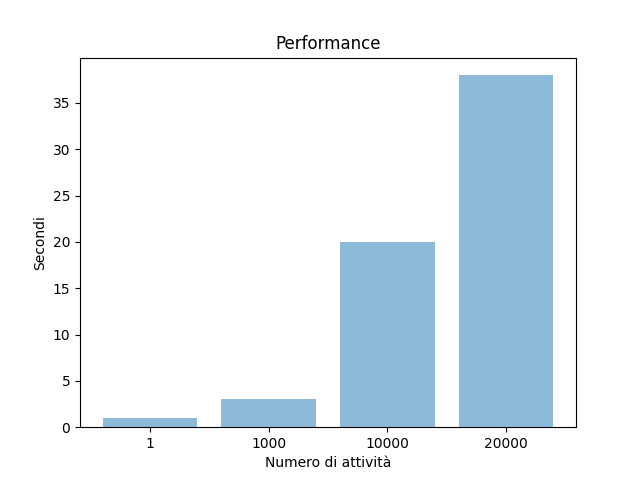
\includegraphics[width =\textwidth]{performance.png}
\caption{Grafico a blocchi}
\end{figure}
Al aumentare delle attività aumenta in maniera quasi lineare il tempo. Questo 
è dovuto al numero alto di cicli di scrittura.
Oltre venti mila attività non è possibile effettuare una stampa perché 
raggiungiamo il limite del buffer di AWS. Se fosse necessario aumentare 
la performance sarebbe sufficiente trasformare le immagini in icone vettoriali.
\\ Altre possibile ottimizzazione potrebbero essere: definire a priori le 
misure del foglio e salvarle come costanti oppure modificare il JSON per 
semplificare la struttura dati. 
Tuttavia non è necessario perché sono tempi ragionevoli.
È più importante notare che il server usi risorse minime, in quanto deve 
solo aspettare il ritorno della chiamata HTTPS. Questo era il fulcro del progetto, 
permettere una migliore e più sicura navigazione alleggerendo il lavoro compiuto 
dal software.
\\ L'implementazione precedente aveva una performance ottima per un numero ridotto 
di informazioni, 
siccome non era legata a dei tempi fissi di connessioni. Allo stesso tempo al 
crescere delle attività aumentava esponenzialmente il tempo e rendeva alto il 
rischio di crash.

\subsection{Aspetto economico}
Il costo della lambda dipende sia dalla potenza della macchina sia dal 
tempo di esecuzione. 
Di default la macchina esegue con 512 MiB di memoria e 128 MiB di archiviazione. 
Naturalmente questa potenza è insufficiente, rallenta estremamente l'esecuzione. 
L'aumento di memoria fissa non influenza in alcun modo la velocità di esecuzione. 
L'allocazione di più memoria, e di conseguenza di potenza di CPU, invece 
genera ottimi risultati. 
\\ Fino a 2 GiB la performance aumenta notevolmente, qualsiasi valore oltre non 
crea nessun aumento degno di nota. 
Facendo una serie di test si è visto che è più conveniente avere la macchina 
meno potente che esegue per periodi più lunghi, piuttosto che una macchina 
estremamente potente che esegue per brevi tratti.
Osservazione intuitiva, siccome c'è una costante di tempo per la creazione 
dell'ambiente. 
A conti fatti si è concordato di tenere una macchina di 1 GiB e 512 MiB di 
memoria fissa. 

\thispagestyle{empty}
\newpage 

\phantomsection
\section*{Conclusione}
\addcontentsline{toc}{section}{Conclusione}
I microservizi offrono un nuovo paradigma di programmazione, uno dove è possibile 
astrarre logica dal proprio software e eseguirla solo qual'ora fosse necessario. 
È possibile condividere questa logica su diversi piattaforme, e permette una 
scalabilità semplice e veloce.
Naturalmente non è adatto a ogni situazione situazione. Una serie di operazioni 
numerose o estremamente lunghe richiedono un servizio. 
Nel caso studiato invece una lambda è estremamente vantaggiosa.
\\ In primo luogo risolve il problema del sovraccarico del server. Migliorare la 
logica e gli algoritmi sarebbe stato corretto ma non avrebbe alleggerito il carico 
di lavoro. L'esportazione del servizio invece permette di mantenere massima 
performance del sito siccome i calcoli vengono fatti altrove.
\\ Il costo temporale non ha subito migliorie nei casi più semplici, ma cresce 
in maniera lineare al aumentare della mole di lavoro. Questo è molto più importante, 
perché ci garantisce usabilità anche nei casi più estremi, visto che non è 
poco comune avere una grossa mole di dati. 
\\ Il progetto si era concentrato sulle stampe più impegnative, siccome erano 
quelle responsabile del impatto negativo sul software e siccome sono le più 
comuni. Non sono però le uniche stampe presenti sul server. Esistono varie 
informazioni da stampare che sono meno vitali e meno usate.
È però corretto avere una logica unica per tutte e portarla su lambda. 
\\ Inoltre non è possibile scaricare solo in formato PDF, bensì anche in XLSX e 
KML. È possibile introdurre queste tipologie in futuro, naturalmente ognuno 
dovrà avere una sua implementazione personale. 
Cosicché ogni operazione di stampa è estratta dal server ed è in un 
unico progetto centrale.
Questo permetterebbe al Rails di concentrarsi esclusivamente sul esposizione
dei dati ai clienti.

\thispagestyle{empty}
\newpage 

\phantomsection
\section*{Bibliografia}
\addcontentsline{toc}{section}{Bibliografia}

\begin{thebibliography}{9}
  \bibitem{}
  AWS documentazione. 
  \url{https://docs.aws.amazon.com/lambda/index.html}

  \bibitem{}
  Ruby documentazione.
  \url{https://ruby-doc.org/}

  \bibitem{}
  Rails documentazione.
  \url{https://api.rubyonrails.org/}

  \bibitem{}
  Nodejs documentazione.
  \url{https://nodejs.org/it/docs}

  \bibitem{}
  Mozilla documentazione.
  \url{https://developer.mozilla.org/en-US/}

  \bibitem{}
  Pdf-kit documentazione.
  \url{https://pdfkit.org/}

  \bibitem{}
  Microservizi wiki.
  \url{https://en.wikipedia.org/wiki/Microservices}

  \bibitem{}
  Cloud computing wiki.
  \url{https://en.wikipedia.org/wiki/Cloud_computing}


  \bibitem{}
  Amazon Web Service wiki.
  \url{https://en.wikipedia.org/wiki/Amazon_Web_Services}

  \bibitem{}
  Remote job entry wiki.
  \url{https://en.wikipedia.org/wiki/Remote_job_entry}

  \bibitem{}
  Amazon aurora.
  \url{https://aws.amazon.com/it/rds/aurora/?nc2=h_ql_prod_fs_aa}

  \bibitem{}
  Amazon DynamoDB
  \url{https://aws.amazon.com/it/dynamodb/?nc2=h_ql_prod_fs_ddb}

  \bibitem{}
  Amazon S3.
  \url{https://aws.amazon.com/it/s3o /?nc2=h_ql_prod_fs_s3}

  \bibitem{}
  Amazon SNS.
  \url{https://aws.amazon.com/it/sns/?nc2=h_ql_prod_ap_sns}

  \bibitem{}
  Amazon SQS.
  \url{https://aws.amazon.com/it/sqs/?nc2=h_ql_prod_ap_sqs}

  \bibitem{}
  Amazon Lambda.
  \url{https://aws.amazon.com/it/lambda/?nc2=h_ql_prod_cp_lbd}

\end{thebibliography}


\end{document}